\chapter{\IfLanguageName{dutch}{Stand van zaken}{State of the art}}
\label{ch:stand-van-zaken}

% Tip: Begin elk hoofdstuk met een paragraaf inleiding die beschrijft hoe
% dit hoofdstuk past binnen het geheel van de bachelorproef. Geef in het
% bijzonder aan wat de link is met het vorige en volgende hoofdstuk.

% Pas na deze inleidende paragraaf komt de eerste sectiehoofding.
\section{\IfLanguageName{dutch}{Global Positioning System (GPS)}{Global Positioning System (GPS)}}
Het Global Positioning System is een wereldwijd gekend systeem, maar toch zijn er heel wat verschillen. Als er gesproken wordt over GPS, wordt er impliciet NAVSTAR bedoeld. Dit is het eerste operationele GPS-systeem dat begonnen was als militaire toepassing. Het is ontwikkeld door de 'United States Air Force'. \autocite{gnss}  Nadien is NAVSTAR toegankelijk gemaakt voor de gewone gebruikers. In deze sectie wordt er toegelicht wat de verschillende systemen zijn en welke gebruikt kunnen worden.

\subsection{\IfLanguageName{dutch}{De werking van GPS}{How GPS works}}
\begin{figure}
	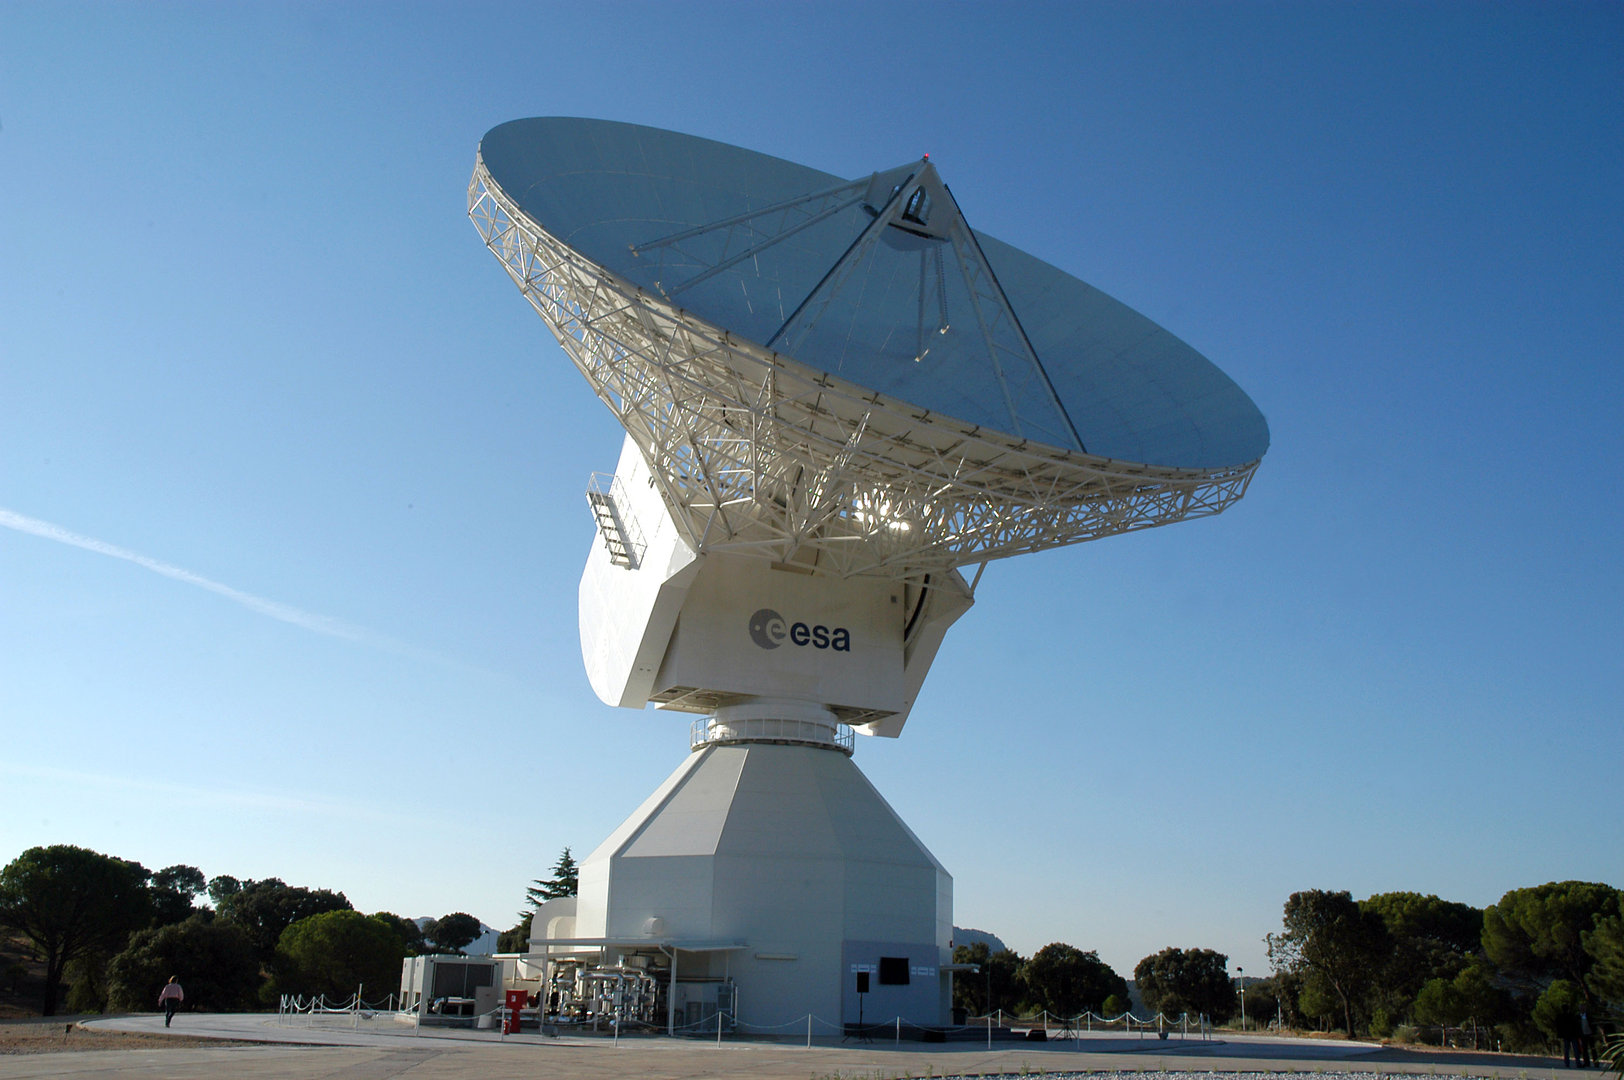
\includegraphics[width=\textwidth,height=\textheight,keepaspectratio]{groundstation.jpg}
	%https://www.google.com/url?sa=i&url=https%3A%2F%2Fwww.esa.int%2FAbout_Us%2FESAC%2FCebreros_ground_station&psig=AOvVaw3m4fRPzsoJEUD7uxKB9P8U&ust=1583062350499000&source=images&cd=vfe&ved=0CAMQjB1qFwoTCJD8uPrU9ucCFQAAAAAdAAAAABAD
	\caption{\href{https://www.esa.int/About_Us/ESAC/Cebreros_ground_stationt}{Voorbeeld Groundstation}}
	\label{fig:groundstation}
\end{figure}
\begin{figure}
	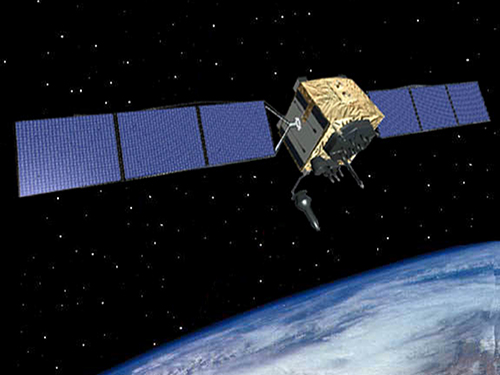
\includegraphics[width=\textwidth,height=\textheight,keepaspectratio]{satelliet.jpg}
	%https://www.google.com/url?sa=i&url=https%3A%2F%2Fspacenews.com%2F40530gps-2f-6-navigation-satellite-slated-to-launch-on-may-15%2F&psig=AOvVaw0tzOggmMim-1CxoYTRl1Ze&ust=1583062792344000&source=images&cd=vfe&ved=0CAMQjB1qFwoTCOD3jc3W9ucCFQAAAAAdAAAAABAD
	\caption{\href{https://spacenews.com/40530gps-2f-6-navigation-satellite-slated-to-launch-on-may-15/}{Voorbeeld GPS-satelliet}}
	\label{fig:satelliet}
\end{figure}

Om een locatie te bepalen zijn er 3 zaken nodig:
\begin{itemize}
	\item Groundstations, deze zijn ontworpen voor buitenplanetaire draadloze communicatie. Ze communiceren door het ontvangen en verzenden van radiogolven met zeer hoge frequentie. (Zie figuur: \ref{fig:groundstation})
	\item Een satelliet, of ook vaak kunstmaan genoemd, is een object dat zich in een baan om een hemellichaam bevindt. \autocite{definitie_satelliet} (Zie figuur: \ref{fig:satelliet})
	\item GPS-ontvanger, dit ontvangt de elektromagnetische signalen van de satellieten.
\end{itemize}

De groundstations worden gebruikt om de locatie bij te houden van de GPS-satellieten. Deze stations worden niet gebruikt voor het bepalen van de huidige locatie van een gebruiker. 
\newline
\newline
De GPS-satellieten broadcasten een signaal uit die de afstand en tijd bevat. Deze tijd wordt berekend met een klok aan boord. Een kwartskristal klok kan na 6 weken een volledige milliseconde afwijken van de werkelijke tijd, wat zeer gevaarlijk is voor ruimteverkeer. Hierdoor maken satellieten gebruik van een ander type klok, de atoomklok. Atoomklokken zijn een 'verbetering' ten opzichte van de kwartskrital klok.  Na 10 jaar wijkt een atoomklok slechts een microseconde af, wat stabieler is in vergelijking met de kwartskristal klok. Alles moet stabiel blijven voor ruimtevaartmisies, waardoor de afwijking van de atoomklok dagelijks gecorrigeerd wordt. \autocite{atomic_clock}
\newline
Als de GPS-ontvanger de tijd en afstand uit het signaal heeft kunnen afleiden, kan het aan de hand van triangulatie zijn locatie bepalen. (Zie figuur: \ref{fig:triangulatie})
Er wordt per satelliet een radius bepaald. Hiervoor zijn minstens drie satellieten nodig. De overlapping van de radiussen bepalen één punt, de locatie van de GPS-ontvanger. Soms kan dit niet accuraat gebeuren, waardoor de radius van een vierde satelliet kan helpen. De laatste radius sluit dan foute mogelijkheden uit waardoor de locatie accurater is. Kortom, hoe meer satellieten, hoe beter de locatiebepaling gebeurd. 

\begin{figure}
	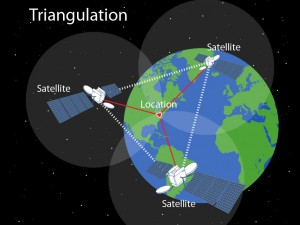
\includegraphics[width=\textwidth,height=\textheight,keepaspectratio]{triangulatie.jpg}
	%https://www.google.com/url?sa=i&url=https%3A%2F%2Fcommunicatiekc.com%2Ftriangulatie%2F&psig=AOvVaw3yrDqiAvEq65KAYiid2aw6&ust=1583063314296000&source=images&cd=vfe&ved=0CAMQjB1qFwoTCKCi68bY9ucCFQAAAAAdAAAAABAD
	\caption{\href{https://communicatiekc.com/triangulatie/}{Werking triangulatie}}
	\label{fig:triangulatie}
\end{figure} 
\pagebreak
\subsection{\IfLanguageName{dutch}{Global Navigation Satellite Systems (GNSS)}{Global Navigation Satellite Systems (GNSS)}}
Als we spreken over het bepalen van onze locatie, gebruiken we altijd de term 'GPS'. Dit is echter niet correct, want er bestaan veel meer technologieën en systemen die hierbij helpen. Iedere technologie wordt verder besproken in dit hoofdstuk.
\newline
Het 'Global Positioning System' is een ruimte gebaseerd navigatiesysteem dat eigendom is van de Verenigde Staten en bestuurd wordt door de 'United States Air Force' (USAF). Officieel heet dit systeem 'Navigation Satellite Time And Ranging' (NAVSTAR). De allereerste versie werd gelanceerd in 1978 en in 1995 operationeel verklaard. GPS is in staat om een ongelimiteerde limiet van gebruikers met een GPS-ontvanger te voorzien van hun locatie op ieder moment van de dag, onafhankelijk van het weer en over de hele wereld. \autocite{gps}
\newline
Naast NAVSTAR bestaat er ook:
\begin{itemize}
	\item Galileo, beheerd door de Europese Unie (EU).
	\item Globalnaya navigatsionnaya sputnikovaya sistema (GLONASS), beheerd door Rusland.
	\item BeiDou Navigation Satellite System (BDS), beheerd door China, ook Compass genoemd.
	\item Indian Regional Navigation Satellite System (IRNSS/NavIC), beheerd door India.
	\item Quasi-Zenith Satellite System (QZSS), beheerd door Japan
\end{itemize}

Er zijn verschillen tussen tussen deze Global Navigation Satellite Systems, namelijk de accuraatheid en het aantal satellieten. Ook zijn QZSS en IRNSS niet bedoeld als globale GPS-systemen. (Zie tabel:\ref{tab:GNSS-vergelijking})
\begin{table}[]
	\begin{tabular}{lll}
		Systeem & Aantal satellieten (actief) & Nauwkeurigheid                                                                        \\
				BDS     & 35                          & 3.6 meter                                                                      \\
		NAVSTAR & 31                          & 3-5 meter                                                                             \\
		GLONASS & 24+                         & 4-10 meter                                                                            \\
		Galileo & 24+                         & 20-50 centimeter                                                                      \\
		IRNSS   & 7                           & \textless 10 meter over India en \textgreater{}20 meter over de Indische Oceaan regio \\
		QZSS    & 7                           & 1 - 0,01 meter                                                                       
	\end{tabular}
\label{tab:GNSS-vergelijking}
\caption{tabel die een vergelijking geeft van alle Global Navigation Satellite Systems}
\autocite{gnss}
\end{table}
\newline
De reden voor het bestaan van deze verschillende systemen is van politieke aard. De EU en Rusland wilden niet afhankelijk zijn van de Verenigde Staten (NAVSTAR).

\section{Verschillende Locatiebepaling-technologieën}
\label{sec:Locatiebepaling-technologieën}
Het bepalen van een positie kan op veel manieren gebeuren. De systemen die besproken werden in de vorige sectie vallen allemaal terug op de traditionele methode, triangulatie. De werking van deze methode wordt in deze sectie verder toegelicht. Naast de traditionele methode is het belangrijk om te weten welke andere opties er nog bestaan. Iedere optie wordt in deze sectie besproken.
\subsection{\IfLanguageName{dutch}{Standard Positioning Service (SPS)}{Standard Positioning Service (SPS)}}
De 'Standard Positioning Service' (SPS) is een positionerings- en timingdienst die signalen broadcast op de GPS L1-frequentie. Deze frequentie, die gebruikt wordt door alle NAVSTAR GPS-satellieten, zorgt ervoor dat GPS vrij te gebruiken is voor iedereen. \autocite{gps}
\newline
Deze vorm van GPS is vrij accuraat, maar presteert minder in vergelijking met het 'Precision Positioning Service'. 
\subsection{\IfLanguageName{dutch}{Precision Positioning Service (PPS)}{Precision Positioning Service (PPS)}}
De 'Precision Positioning Service' (PPS) is een  positionerings- en timingdienst die signalen broadcast op de GPS L1 en L2 frequenties. Het functioneert hetzelfde als SPS, maar hierbij wordt er ook gebruik gemaakt van een precisiecode (P) die alleen beschikbaar is voor geautoriseerde gebruikers. Hiermee wordt voornamelijk het Amerikaans leger en zijn allianties bedoeld. \autocite{pps} Voor september 2007 werd er gebruik gemaakt van 'Selective Availability' (SA). Zo kon het leger van de Verenigde Staten de accuraatheid bewust degraderen voor veiligheidsredenen. De nieuwere GPS III-satellieten zouden niet meer uitgerust zijn met de SA-functie. 
\newline
Deze service wordt voor de proof of concept niet gebruikt omdat het  ontoegankelijk is voor gewone burgers.
\subsection{\IfLanguageName{dutch}{Differential Global Positioning System (DGPS)}{Differential Global Positioning System (DGPS)}}
Differential Global Positioning System (DGPS) verbetert de accuraatheid van GPS. Dit systeem maakt gebruik van correctietechnieken. Deze technieken kunnen real-time gebeuren, maar ook na het bepalen van de locatie. DGPS vereist een GPS-ontvanger (referentiestation/basestation) wiens locatie gekend is (fixed). De referentie gaat zijn locatie herberekenen en berekent het verschil tussen de gekende locatie en de berekende locatie. Het verschil wordt als volgt toegepast op de GPS-ontvanger zijn berekende locatie. Deze techniek resulteert in een betere locatiebepaling voor de tweede GPS-ontvanger. \autocite{dgps} (Zie figuur:\ref{fig:dgps})
\begin{figure}
	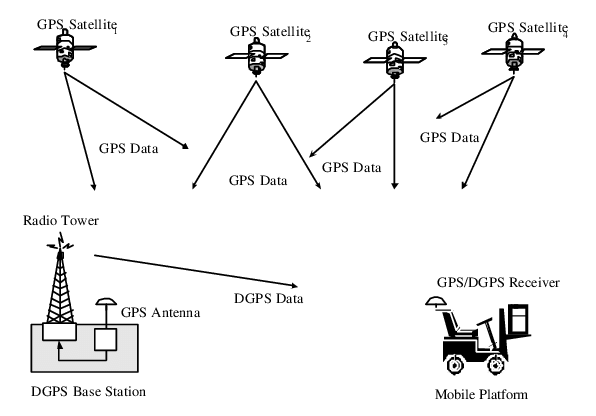
\includegraphics[width=\textwidth,height=\textheight,keepaspectratio]{dgps.png}
		%https://www.google.com/url?sa=i&url=https%3A%2F%2Fwww.researchgate.net%2Ffigure%2FComponents-of-a-DGPS-System_fig1_252064818&psig=AOvVaw07YsVmaU9ifoTgAxmkFPSb&ust=1583073831676000&source=images&cd=vfe&ved=0CAMQjB1qFwoTCPCjlt7_9ucCFQAAAAAdAAAAABAD
	\caption{\href{https://www.researchgate.net/figure/Components-of-a-DGPS-System_fig1_252064818}{Differential Global Positioning System}}
	\label{fig:dgps}
\end{figure}
\newline
De 'Flemish Positioning Service' (FLEPOS) maakt ook gebruik van deze techniek. Het FLEPOS 3.0-netwerk bestaat momenteel uit 45 GNSS-referentiestations, waarvan 33 referentiestations in eigen beheer. Het gebruik hiervan is gratis indien de aanvraag voor een abonnement is goedgekeurd. Deze referentiestations bevinden zich in België, Nederland, Frankrijk, Duitsland en Engeland.
\newline
Door het beperkt aantal referentiestations kan deze methode niet geïmplementeerd worden binnen de proof of concept, omdat het bereik niet globaal genoeg is.
\subsection{\IfLanguageName{dutch}{Wide Area Augmentation System (WAAS)}{Wide Area Augmentation System (WAAS)}}
'Wide Area Augmentation' (WAAS) kan ,naast basestations op aarde (DGPS), ook GEO-satellieten gebruiken als vaste referentiepunten. Deze satellieten bevinden zich op 36.000 km hoogte boven de evenaar en draaien rond op dezelfde snelheid als de aarde. Hierdoor blijft de positie van de geosatelliet stationair ten opzichte van de aarde, waardoor het gebruikt kan worden als referentiestation.(Zie figuur:\ref{fig:geostationair})
\begin{figure}
	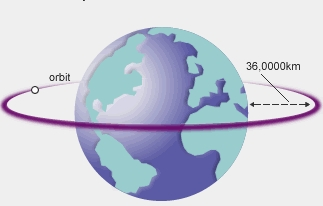
\includegraphics[width=\textwidth,height=\textheight,keepaspectratio]{geostationair.png}
	%https://aardrijkskunde.dbz.be/graad3/taken/oefening_satellieten.htm
	\caption{\href{https://aardrijkskunde.dbz.be/graad3/taken/oefening_satellieten.htm}{Geostationair}}
	\label{fig:geostationair}
\end{figure}
\subsection{\IfLanguageName{dutch}{Assisted Global Positioning System (A-GPS)}{Assisted Global Positioning System (A-GPS)}}
Een GPS-toestel kan er enkele minuten over doen om je locatie te bepalen. Deze verloren tijd heet 'Time To First Fix' (TTFF). De duur van deze TTFF hangt af van je locatie en storing. Een open veld zal een kleinere TTFF hebben dan een stad. Assisted Global Positioning (AGPS/A-GPS/aGPS) verkleint de TTFF. 
\newline
Gsm masten hebben GPS-ontvangers die voortdurend informatie van GPS-satellieten verzamelen. Op deze informatie worden allerlei bewerkingen uitgevoerd en als volgt opgeslagen in een database. Dit heeft enkele voordelen voor de gsm die zijn locatie probeert te bepalen:
\begin{itemize}
	\item Snellere locatie bepaling;
	\item Minder computerkracht nodig;
	\item Minder batterijverbruik;
	\item Mogelijkheid om de locatie indoor te bepalen.
\end{itemize} 
Andere voordelen zijn hoge accuraatheid (5-50 meter) en er zijn slechts twee waarneembare GPS-satellieten nodig.
Opmerkelijk is dat de accuraatheid minder goed is in vergelijking met het zelf bepalen van de locatie (Zie: \ref{tab:GNSS-vergelijking}). Er zullen field tests en metingen worden uitgevoerd om deze stellingen te controleren. \autocite{agps}
\subsection{\IfLanguageName{dutch}{Advanced Mobile Location (AML)}{Advanced Mobile Location (AML)}}
Tot nu toe was er nog geen enkele techniek die de exacte locatie kon bepalen. 'Advanced Mobile Location' (AML) is de nieuwste (open source) techniek die hiervoor een oplossing biedt. Het maakt gebruik van:
\begin{itemize}
	\item wifi
	\item sms
	\item GNSS
\end{itemize}
Door gebruik te maken van bovenstaande positioneringstechnieken is het de meest accurate en tegelijkertijd de traagste methode van alle besproken methodes. 
\newline
Deze methode wordt gebruikt bij noodtelfoon oproepen. Bij het begin van het bellen wordt er eerst gekeken of de Wifi en GPS aanstaat. Als de 'battery check' positief is, worden deze services aangezet indien ze nog niet aanstonden. 
\newline
AML gaat parallel zijn locatie proberen bepalen aan de hand van wifi, sms en GNSS, zodat het zo min mogelijk tijd verliest om de beller te lokaliseren. De lokatiebepaling gebeurt aan de hand van een geprioritiseerde rij. Indien GNSS als eerste de lokatie kan bepalen wordt dit als eerst verzonden naar de hulpdiensten. 
Als tweede optie wordt de lokatie bepaald met behulp van wifi. Hierbij wordt de locatie gebaseerd op wifi 'Service Set Identifiers' (SSIDs) of MAC-adressen van access points waarmee de gsm verbonden is. Als laatste optie wordt de cell ID verstuurd van de mast waarmee de beller verbonden is. Indien men geen lokatie kan bepalen, wordt er een sms verstuurd dat alle positioneringstechnieken (wifi, GNSS, cell ID) gefaald hebben.
\newline
In 2020 zijn er nog steeds slechts 19 landen wereldwijd die AML implementeren. AML kan alleen gebruikt worden bij het bellen van het noodnummer. De proof of concept werkt alleen met je eigen nummer, waardoor AML geen optie is. \autocite{aml} Ook is het bellen van het noodnummer zonder noodgeval illegaal.
\subsection{\IfLanguageName{dutch}{General Packet Radio Service (GPRS)}{General Packet Radio Service (GPRS)}}
General Packet Radio Service (GPRS) is een totaal andere manier voor locatiebepaling. Deze technologie vereist geen GPS, maar wel roaming. Deze verbinding haalt de locatie op van zendmasten, waardoor je via triangulatie je locatie kan bepalen (Zie figuur:\ref{fig:triangulatie_gprs}). Deze techniek werkt hetzelfde als GPS.
\newline
Een nadeel van deze technologie is dat het veel minder accuraat is. Volgens \cite{gprs} kan dit variëren van 20 tot 50 meter. Het voordeel aan GPRS is dat het in staat is via roaming of sms zijn locatie te delen. Het gebruik van sms zorgt ervoor dat de proof of concept op een zeer globale manier gebruikt kan worden. Ook is het een goedkopere optie, want sms-en zijn voor providers zo goed als gratis in tegenstelling tot mobiele data. De combinatie van een GPS-ontvanger (ondersteuning voor NAVSTAR, Galileo en GLONASS) en de mogelijkheid tot het versturen van een sms zou zorgen voor een ideale proof of concept. 
\begin{figure}
    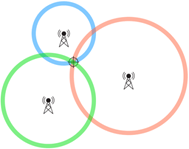
\includegraphics[width=\textwidth,height=\textheight,keepaspectratio]{triangulatie_gprs.png}
%https://www.google.com/search?tbs=simg:CAQSrQEJrrLXpgtW1nYaoQELELCMpwgaYgpgCAMSKJkIsBTyEoIDmgiDA5cIgQO5B4gDmj2dPaE0_1zO2J9A2-DP5M8U9yzcaMJJQwz9JWeZp5PeQ91p9B_1t-s-t57GaZYKqFkjHWNDErGPjWTFiDfGTdUPZPzFLx_1SAEDAsQjq7-CBoKCggIARIEyZLpqAwLEJ3twQkaGgoYCgZjaXJjbGXapYj2AwoKCC9tLzAxdmtsDA&sxsrf=ALeKk02ZKs3-33pizx_yPs1LYQ2NzzRrMw:1583058379858&q=trianguleren+mobiel&tbm=isch&sa=X&ved=2ahUKEwjJ_46DiPnnAhWNLewKHREFBhEQwg4oAHoECAcQKA
    \caption{\href{http://bigpicturequestions.com/how-does-triangulation-help-our-evolution/}{Trangulatie bij GPRS}}
    \label{fig:triangulatie_gprs}
\end{figure}
\pagebreak
\raggedbottom
\section{\IfLanguageName{dutch}{Ongunstige omstandigheden}{Unfavorable circumstances}}
De proof of concept moet blijven functioneren in ongunstige omstandigheden, zoals sneeuw en water. Het moet in staat zijn om te functioneren als GPS-ontvanger op een surfboard en als lawinepieper. In deze sectie wordt onderzocht aan welke voorwaarden de proof of concept moet voldoen.
\subsection{\IfLanguageName{dutch}{Water}{Water}}
Het grooste probleem voor GPS-ontvangers is dat ze niet kunnen functioneren onder water. Dit komt doordat de sterkte van het signaal te snel afneemt onder water. Hetzelfde geldt voor mobiel netwerk, want beiden zijn elektromagnetische golven. \autocite{underwater} Er is ook een verschil tussen zout en zoetwater. Het zout in zeewater versterkt het geleidend effect waardoor GPS-signalen nog minder presteren in zeewater dan in zoetwater. Voor de proof of concept is dit geen struikelblok, indien het wordt toegepast op surfboards. Surfboards zijn zodanig gemaakt dat ze altijd blijven drijven, waardoor de proof of concept zal blijven functioneren naar behoren.
\subsection{\IfLanguageName{dutch}{Sneeuw}{Snow}}
In tegenstelling tot water, blijven GPS-signalen wel functioneren onder sneeuw tot een zekere diepte. Een GPS-signaal die passeert door lawine puin zal onderworpen worden aan verschillende effecten zoals verzwakking, reflectie, verstrooiing, breking, multipad en vervagen. (Zie figuur:\ref{fig:avalanche}) Sneeuw is net als water een geleidend materiaal, waardoor het (L1 band) GPS-signaal verzwakt. De verzwakking hangt af van de hoeveelheid water in sneeuw. Bijvoorbeeld een GPS-signaal kan tot 400 meter diep gaan bij sneeuw met een massadichtheid van 0.3 g/cm\textsuperscript{3}. Bij sneeuw waarvan water 1 percent van het volume opmaakt, penetreert het GPS-signaal slechts 3 meter.
\autocite{avalanche_gps} Hieruit wijst dat de proof of concept ook mogelijks kan dienen als een lawinepieper. 
\begin{figure}
    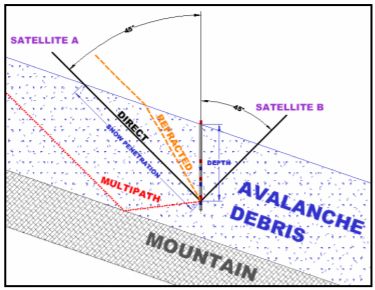
\includegraphics[width=\textwidth,height=\textheight,keepaspectratio]{avalanche.png}
    %https://www.researchgate.net/figure/Signal-Paths-in-Avalanche-Debris_fig1_253280455
    \caption{\href{https://www.researchgate.net/figure/Signal-Paths-in-Avalanche-Debris_fig1_253280455}{Signaal paden bij lawine puin}}
    \label{fig:avalanche}
\end{figure}
\pagebreak
\section{\IfLanguageName{dutch}{Toestellen}{Devices}}
Voor de proof of concept werd er goed nagedacht welke Locatiebepaling-technologieën gebruikt kunnen worden. Naast bruikbaar in ideale omstandigheden, moet het ook in ongunstige omstandigheden kunnen blijven functioneren. Ook moet er voldaan worden aan de volgende vereisten:
\begin{itemize}
    \item Mogelijkheid tot het bepalen van de locatie;
    \item Mogelijkheid tot het delen van de locatie via sms;
    \item Mogelijkheheid tot het delen van de locatie via roaming;
    \item Mogelijkheid om te werken op batterij;
    \item Mogelijkheid tot waterdichtheid;
    \item Zo goedkoop mogelijk blijven.
\end{itemize}
Naast deze eisen moet de batterijduur zo lang mogelijk meegaan en de locatiebepaling moet zo accuraat mogelijk zijn.
\subsection{\IfLanguageName{dutch}{Raspberry Pi}{Raspberry Pi}}
Er bestaan verschillende veries van de Raspberry Pi. De versies die in aanmerking komen zijn:
\begin{itemize}
    \item Raspberry Pi 4 Model B (39.95 euro);
    \item Raspberry Pi 3 A+ (26.80 euro);
    \item Raspberry Pi 3 B+ (39.95 euro);
    \item Raspberry Pi 3 B (37.95 euro).
\end{itemize}
(de prijzen zijn geraadpleegd op: \url{https://www.raspberrypi.org/products})
\newline
Naast de Raspberry Pi zijn er nog componenten nodig (zie tabel:\ref{tab:rpi}).
\begin{table}[]
	\begin{tabular}{llll}
		\textbf{Component}           & \textbf{Prijs (euro)} & \textbf{Doel}                                                                & Link                                                                                                                                                                                                                             \\
		\href{https://www.raspberrypi.org/products}{Raspberry Pi 3A+}    & 26.80        & Het hoofd toestel, draait een besturingssysteem en voert alles aan. & https://www.raspberrypi.org/products                                                                                                                                                                                             \\
		\href{https://www.bol.com/nl/p/ philips-sd-kaart-8gb-sd-card-class-4/9200000023935849/?country=BE\&Referrer=ADVNLPPcefd2c00d536683c00927aff17000051123\& utm\_source=51123\&utm\_medium=Affiliates\&utm\_campaign=CPS\&utm\_content=txl}{SD-kaart (min. 8GB)} & 9.99         & Hierop wordt het besturingssysteem en het script opgeslagen.        & https://www.bol.com/nl/p/ philips-sd-kaart-8gb-sd-card-class-4/9200000023935849/?country=BE\&Referrer=ADVNLPPcefd2c00d536683c00927aff17000051123\& utm\_source=51123\&utm\_medium=Affiliates\&utm\_campaign=CPS\&utm\_content=txl \\
		\href{https://www.robotshop.com/eu/ en/gsm-gprsgnssbluetooth-hat-raspberry-pi.html}{GSM HAT}             & 46.61        & Dit zorgt voor online communicatie om de data door te sturen.       & https://www.robotshop.com/eu/ en/gsm-gprsgnssbluetooth-hat-raspberry-pi.html                                                                                                                                                     \\
		\href{https://www.sossolutions.nl/1566-usb-battery-pack-for-raspberry-pi-10000mah-2-x-5v-outputs?gclid=CjwKCAjwvZv0BRA8EiwAD9T2VfLwMiBk7S2IyG0X13mIPVppguIaRPsgBf2mtAYpxLGU7K8PmdalmRoCbZgQAvD\_BwE}{5V} Battery          & 54.95        & Hierdoor kan de proof of concept draadloos werken.                  & https://www.sossolutions.nl/1566-usb-battery-pack-for-raspberry-pi-10000mah-2-x-5v-outputs?gclid=CjwKCAjwvZv0BRA8EiwAD9T2VfLwMiBk7S2IyG0X13mIPVppguIaRPsgBf2mtAYpxLGU7K8PmdalmRoCbZgQAvD\_BwE                                    \\
		\href{https://www.sossolutions.nl/raspberry-pi-gps-hat?gclid=CjwKCAjwvZv0BRA8EiwAD9T2VZeOJ8Gh0lykmCo9hwT2Zn5j8bvYHn\_mQX2lXPTCSkvUFwH6F3qQexoCutYQAvD\_BwE}{GPS HAT}             & 39.95        & Een meer accurate lokatiebepaling in vergelijking met AGPS.         & https://www.sossolutions.nl/raspberry-pi-gps-hat?gclid=CjwKCAjwvZv0BRA8EiwAD9T2VZeOJ8Gh0lykmCo9hwT2Zn5j8bvYHn\_mQX2lXPTCSkvUFwH6F3qQexoCutYQAvD\_BwE                                                                             \\
		Totale kost:        & \textbf{178.30}        &                                                                     &                                                                                                                                                                                                                                 
	\end{tabular}
\caption{Prijs opstelling Raspberry Pi}
\label{tab:rpi}
\end{table}

\subsection{\IfLanguageName{dutch}{Arduino}{Arduino}}
Naast de Raspberry Pi is er de mogelijkheid om gebruik te maken van een Arduino. Arduino heeft een module die geprogrammeerd kan worden om te voldoen aan alle eisen, namelijk de MKR 1400 GSM module. (Zie figuur: \ref{fig:mkr1400}) Er zijn uiteraard nog componenten nodig (zie tabel: \ref{tab:arduino}).
\begin{table}[]
	\begin{tabular}{llll}
		\textbf{Component}         & \textbf{Prijs (euro)} & \textbf{Doel}                                                               & Link                                                                     \\
		\href{https://store.arduino.cc/arduino-mkr-gsm-1400-1415}{MKR GSM}           & 80.35        & Dit component runt het script en stuurt de andere componenten aan. & https://store.arduino.cc/arduino-mkr-gsm-1400-1415                       \\
		\href{https://store.arduino.cc/arduino-mkr-gps-shield}{MKR GPS Shield}    & 41.75        & Een meer accurate lokatiebepaling in vergelijking met AGPS.        & https://store.arduino.cc/arduino-mkr-gps-shield                          \\
		\href{https://www.kiwi-electronics.nl/lithium-ion-polymer-battery-3-7v-2500mAh}{LiPo 3.7V 2500mAh} & 25.90        & Dit zorgt ervoor dat het MKR board draadloos kan werken.           & https://www.kiwi-electronics.nl/lithium-ion-polymer-battery-3-7v-2500mAh \\
		Totale kost:      & \textbf{148.00}       &                                                                    &                                                                         
	\end{tabular}
\caption{Prijs opstelling Arduino}
\label{tab:arduino}
\end{table}

\begin{figure}
    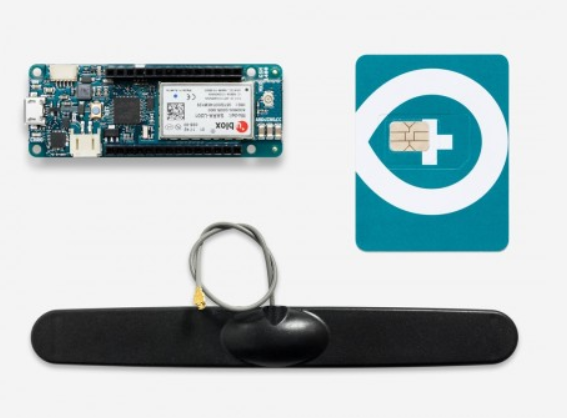
\includegraphics[width=\textwidth,height=\textheight,keepaspectratio]{mkr1400gsm.png}
    %https://store.arduino.cc/arduino-sim-mkr-gsm-1400-cellular-kit-1417?fbclid=IwAR0kJk6t6PVON-YakV_EiSOnb5y2RgBRQW0c6pVmpRw-hJlPRHO99qDdjSA
    \caption{\href{https://store.arduino.cc/arduino-sim-mkr-gsm-1400-cellular-kit-1417?fbclid=IwAR0kJk6t6PVON-YakV_EiSOnb5y2RgBRQW0c6pVmpRw-hJlPRHO99qDdjSA}{Arduino MKR 1400 GSM module}}
    \label{fig:mkr1400}
\end{figure}

\subsection{Proof of concept}
De proof of concept bestaat uit de MKR 1400 GSM Module met een MKR GPS Shield. Deze optie is gekozen, omdat het goedkoop en klein is. Ook heeft de MKR 1400 GSM module (microcontroller) een beter batterijverbruik ten opzichte van de Raspberry Pi (computer).
\newline
De kleine schaal van de MKR 1400 GSM module is een goede reden om dit te gebruiken voor de proof of concept. Hierdoor kan er een robuuste, duurzame en waterbestendige casing gemaakt worden. De casing zou geprint worden met behulp van een 'Anycubic 3D' printer. Zo is er de mogelijkheid om een volledig eigen ontwerp te gebruiken zoals een vin op een surfboard (GPS-ontvanger) of een binding op een snowboard (lawinepieper). Het filament dat gebruikt zou worden is nylon of PETG. Beide voldoen aan de eisen van de casing.